\section{Implementation results at the current snapshot}
\subsection{Completed U-Net training and evaluation}
The U-Net experiment completed 23 epochs and stopped after eight consecutive epochs without an improved validation foreground mIoU. Its selected checkpoint is epoch 15. This includes an epoch-boundary continuation from epoch 7 after host kernel/RAM descriptors changed; the continuation retains the same experiment, seed and budget.

Figure~\ref{fig:unetcurves} shows training loss decreasing from 1.5083 at epoch 1 to 0.6102 at epoch 23 while training foreground mIoU rises from 0.0132 to 0.4072. Validation foreground mIoU peaks at 0.053085 at epoch 15; its final value is 0.047450. Validation loss is lowest at epoch 5 (1.271954) and ends at 1.516843. The growing train--validation gap is consistent with overfitting in this run, without establishing a single cause.
\begin{figure}[H]\centering
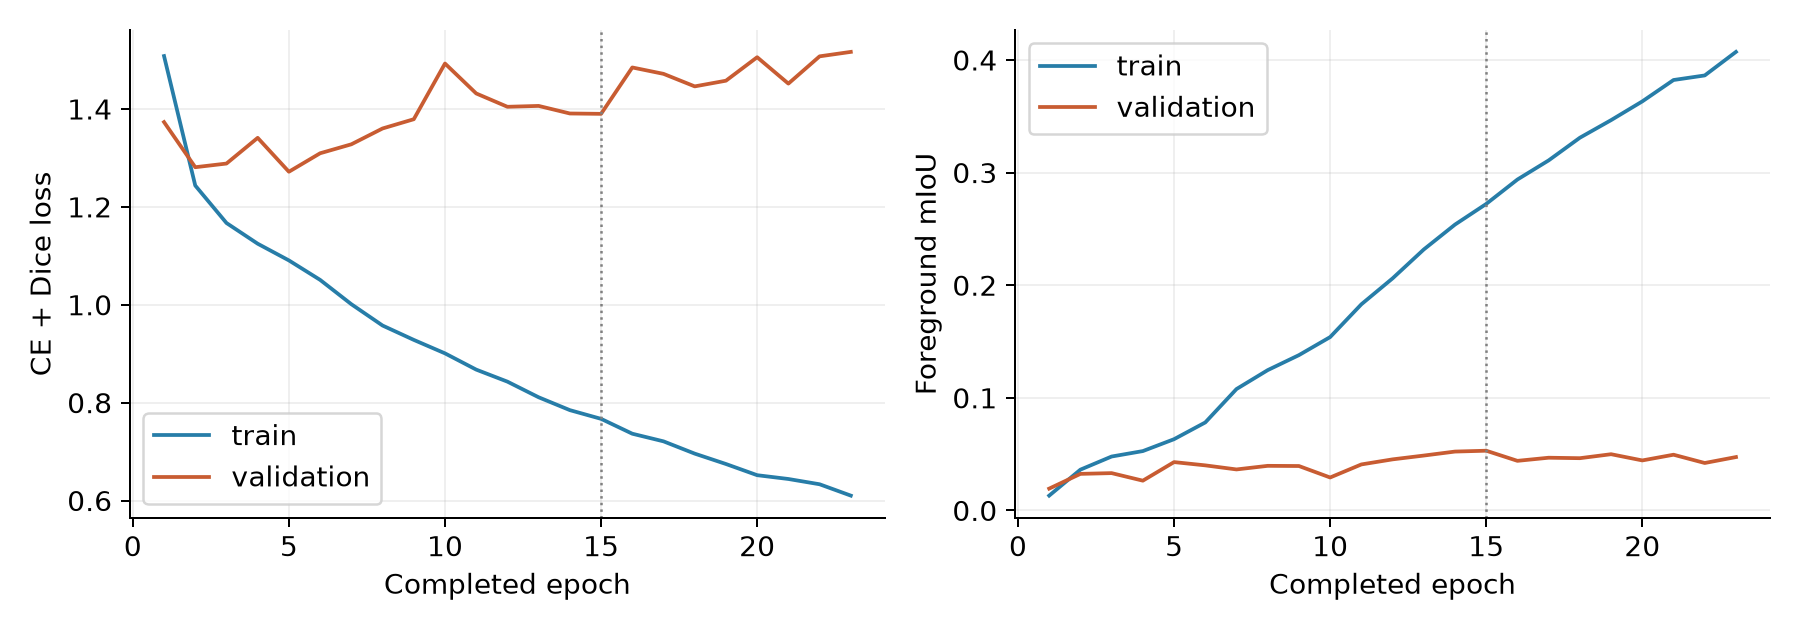
\includegraphics[width=\textwidth]{images/unet_curves.png}
\caption{Completed U-Net history. The dotted line marks the validation-selected epoch 15; the run ends at epoch 23.}\label{fig:unetcurves}
\end{figure}
The metric used to choose the checkpoint is foreground mIoU, so minimum validation loss and selected epoch need not coincide.

The selected checkpoint was replayed on validation and evaluated on all 1,078 test images. Table~\ref{tab:metrics} places these completed U-Net scores next to S0's best-so-far validation score, while retaining the different execution states.
\begin{table}[H]
\centering\small
\caption{Measured metrics at epoch 15. U-Net is a completed run; S0 is a15-epoch partial snapshot. All scores are on a0--1 scale.}\label{tab:metrics}
\begin{tabular}{lrrr}\toprule
Metric & U validation & U test & S0 validation \\ \midrule
Foreground mIoU & 0.053085 & 0.035627 & 0.195336 \\
Foreground Dice & 0.084369 & 0.058519 & 0.280506 \\
Trash mIoU & 0.032704 & 0.014652 & 0.137865 \\
All-class mIoU & 0.103646 & 0.087050 & 0.239732 \\
All-class Dice & 0.135542 & 0.111123 & 0.321323 \\
CE + Dice loss & 1.390246 & 1.407840 & 1.134105 \\
Valid pixels (M) & 176.765 & 186.340 & 176.765 \\
Ignored pixels (\%) & 37.39 & 34.06 & 37.39 \\
\bottomrule\end{tabular}
\end{table}

U-Net test foreground mIoU is 0.035627, foreground Dice 0.058519 and trash mIoU 0.014652. Its validation-to-test foreground mIoU difference is 0.017458. These are observations for a single seed and fixed split, rather than estimates of variability across repeated runs.

\subsection{Measured SegFormer pilots}
Both SegFormer arms completed 20 optimization steps on a fixed real training batch before their main configurations were frozen. Table~\ref{tab:pilots} records finite-loss, gradient and capacity diagnostics. Each pilot's final loss is lower than its initial loss, and peak reserved CUDA memory remains below 90\% of GPU memory.
\begin{table}[H]
\centering\small
\caption{Measured 20-step, fixed-train-batch diagnostics on the T4. These are capacity/gradient checks, not held-out segmentation results.}\label{tab:pilots}
\begin{tabular}{lrrrr}\toprule
Arm & First loss & Last loss & Peak reserved (GiB) & GPU memory (GiB) \\ \midrule
S0 & 3.8140 & 3.0349 & 2.70 & 14.56 \\
S1 & 3.8145 & 3.0304 & 2.73 & 14.56 \\
\bottomrule\end{tabular}
\end{table}

Pilot models are discarded; main training starts again from the prescribed pretrained checkpoint and seed. The similar pilot losses do not measure the effect of augmentation on held-out segmentation. Pilot memory is also not a measurement of peak memory across the complete main-training workload.

\subsection{S0 main-training progress: 15 completed epochs}
The supplied S0 checkpoint/history contains 15 completed epochs, below the configured 40-epoch limit. Epoch 15 is currently best, and the early-stopping counter is zero. Therefore the snapshot is \textbf{an incomplete main run}, not a completed 40-epoch or early-stopped SegFormer experiment.

Figure~\ref{fig:s0 curves} shows the available S0 history. Training loss falls from 1.250555 at epoch 1 to 0.247658 at epoch 15, and training foreground mIoU rises from 0.084281 to 0.744726. Validation foreground mIoU rises from 0.100556 to its current maximum 0.195336. At epoch 15, validation Dice is 0.280506, trash mIoU 0.137865 and loss 1.134105.
\begin{figure}[H]\centering
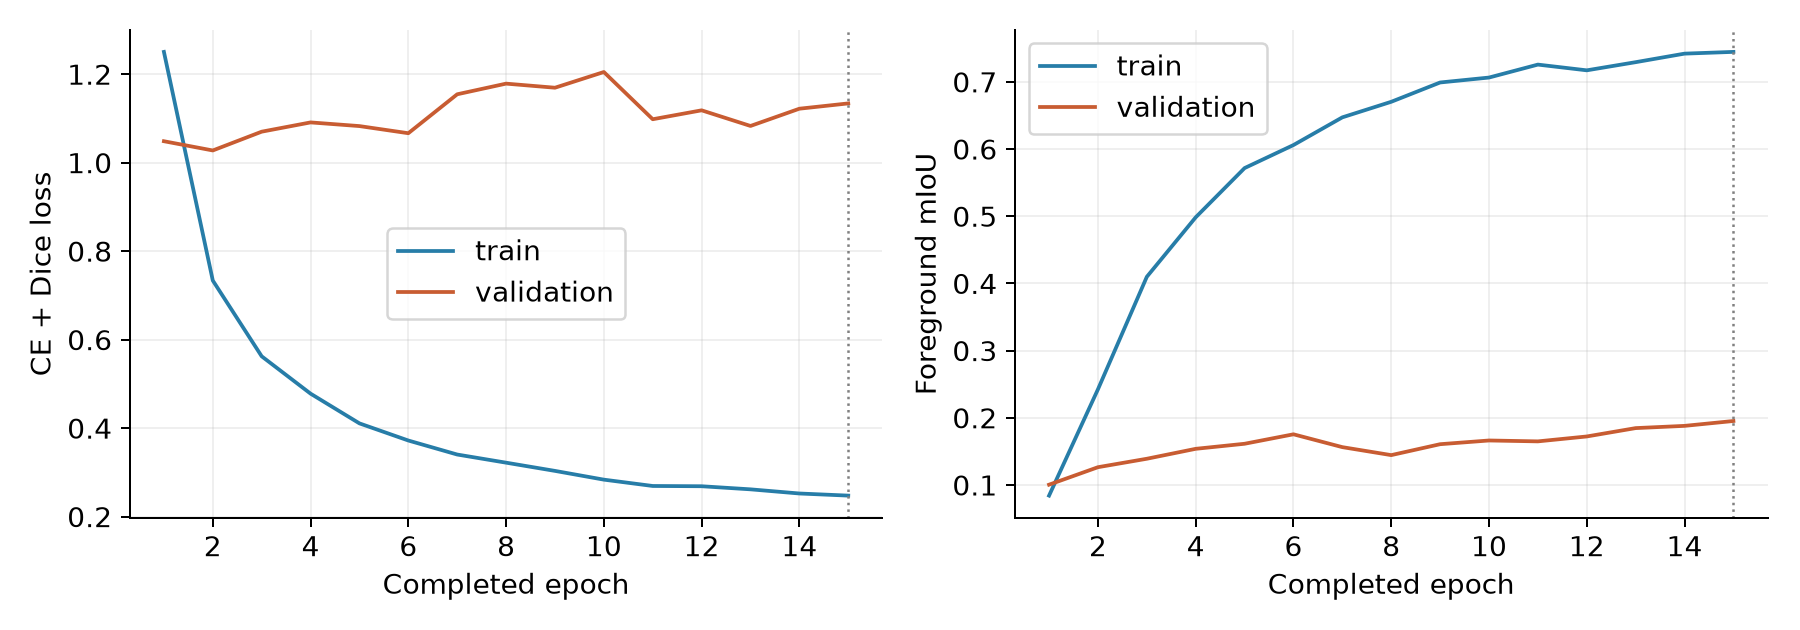
\includegraphics[width=\textwidth]{images/segformer_s0_curves.png}
\caption{Partial SegFormer S0 history through epoch 15. The selected epoch is best-so-far; training has not reached its completion criterion.}\label{fig:s0 curves}
\end{figure}
The latest train--validation foreground mIoU gap is 0.549390. Validation loss reached its lowest observed value at epoch 2 (1.027752), whereas foreground mIoU is highest at epoch 15. Better hard-mask overlap and lower probabilistic loss need not occur together; the saved foreground-mIoU selection rule remains unchanged. The large training/validation gap motivates continued scrutiny of class generalization, rather than treating the training score as held-out quality.

The partial S0 validation mIoU exceeds the completed U-Net validation mIoU by 0.142251 (14.2251 percentage points). This comparison uses the same validation membership and scoring convention. It is evidence that the current S0 configuration learns useful foreground structure; architecture, initialization, learning rate and execution progress differ, so it is neither a final ranking nor a controlled estimate of pretraining's contribution. No S0 test score or independent best-checkpoint validation replay is included in the supplied snapshot; the S0 values come from completed epoch validation in the training history.

\subsection{Per-class overlap and error patterns}
Table~\ref{tab:perclass} preserves each class's measured overlap, and Figure~\ref{fig:classcompare} compares only the two validation columns. The U test column remains a separate completed held-out evaluation.
\begin{table}[H]
\centering\small
\caption{Class-wise overlap. S0 columns use its best-so-far validation checkpoint; no S0 test result is claimed.}\label{tab:perclass}
\begin{tabular}{rlrrrr}\toprule
ID & Class & U val IoU & U test IoU & S0 val IoU & S0 val Dice \\ \midrule
0 & \cls{background} & 0.9126 & 0.9098 & 0.9501 & 0.9744 \\
1 & \cls{rov} & 0.4722 & 0.3564 & 0.6907 & 0.8171 \\
2 & \cls{plant} & 0.0190 & 0.0038 & 0.1074 & 0.1940 \\
3 & \cls{animal_fish} & 0.0162 & 0.0367 & 0.5031 & 0.6694 \\
4 & \cls{animal_starfish} & 0.0000 & 0.0000 & 0.0323 & 0.0627 \\
5 & \cls{animal_shells} & 0.0000 & 0.0000 & 0.0000 & 0.0000 \\
6 & \cls{animal_crab} & 0.0804 & 0.0292 & 0.2820 & 0.4399 \\
7 & \cls{animal_eel} & 0.0000 & 0.0268 & 0.4068 & 0.5784 \\
8 & \cls{animal_etc} & 0.0000 & 0.0000 & 0.0000 & 0.0000 \\
9 & \cls{trash_etc} & 0.0802 & 0.0325 & 0.0575 & 0.1088 \\
10 & \cls{trash_fabric} & 0.0358 & 0.0145 & 0.0729 & 0.1359 \\
11 & \cls{trash_fishing_gear} & 0.0000 & 0.0000 & 0.0078 & 0.0155 \\
12 & \cls{trash_metal} & 0.0390 & 0.0036 & 0.0618 & 0.1163 \\
13 & \cls{trash_paper} & 0.0000 & 0.0000 & 0.1849 & 0.3121 \\
14 & \cls{trash_plastic} & 0.0901 & 0.0666 & 0.2474 & 0.3966 \\
15 & \cls{trash_rubber} & 0.0000 & 0.0000 & 0.0012 & 0.0024 \\
16 & \cls{trash_wood} & 0.0166 & 0.0000 & 0.4694 & 0.6389 \\
\bottomrule\end{tabular}
\end{table}

S0's strongest foreground validation IoUs at epoch 15 are ROV 0.6907, animal fish 0.5031, trash wood 0.4694 and animal eel 0.4068. Animal shells and animal other still have zero validation IoU. Improvement is not uniform: trash other has S0 validation IoU 0.0575 compared with U-Net 0.0802. A higher macro score therefore does not imply every debris category has improved.
\begin{figure}[H]\centering
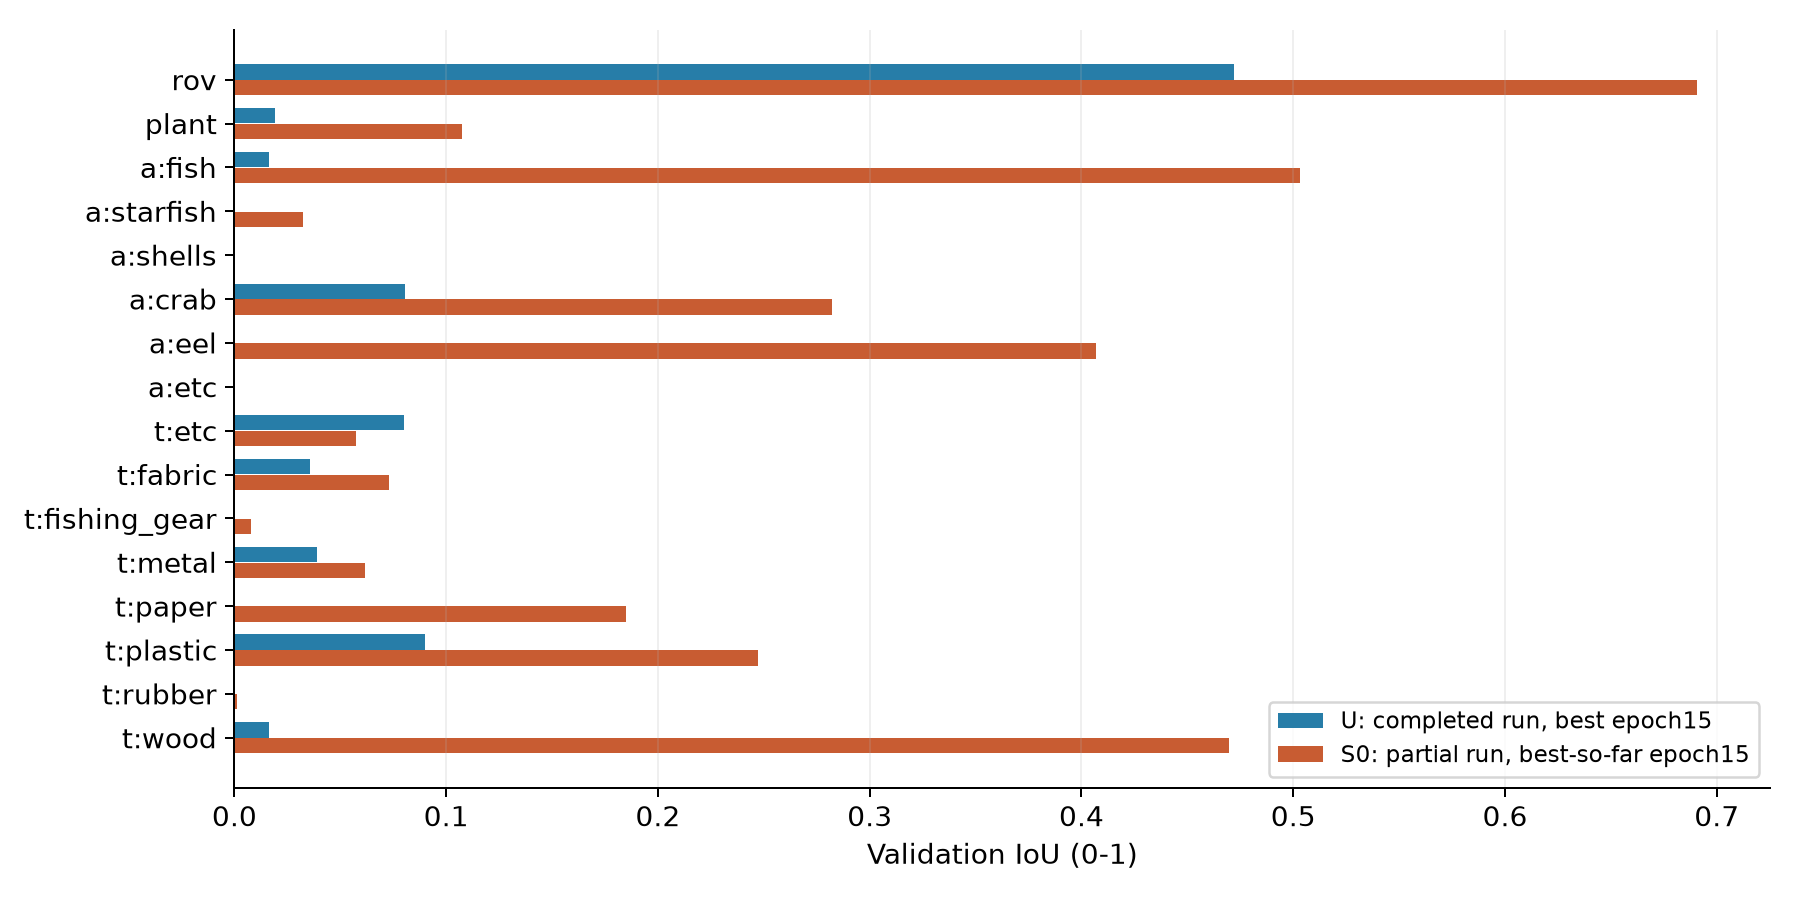
\includegraphics[width=\textwidth]{images/validation_per_class.png}
\caption{Validation IoU by foreground class. U is a completed run and S0 is partial; both columns refer to epoch 15. Prefixes a:/t: denote animal/trash.}\label{fig:classcompare}
\end{figure}
The U-Net test result remains weak across many categories: six foreground classes have zero IoU, and its strongest foreground class is ROV (0.3564). Sparse support is a plausible contributor, but aggregate counts do not distinguish class imbalance, appearance shift, boundary errors and optimization effects as causes.

To show how these errors are distributed, Figure~\ref{fig:confusion} normalizes each confusion row by its true-class support. This puts frequent and rare categories on a common within-class scale. The left panel is U test; the right is S0 validation, so the panels are not a same-partition model comparison.
\begin{figure}[H]\centering
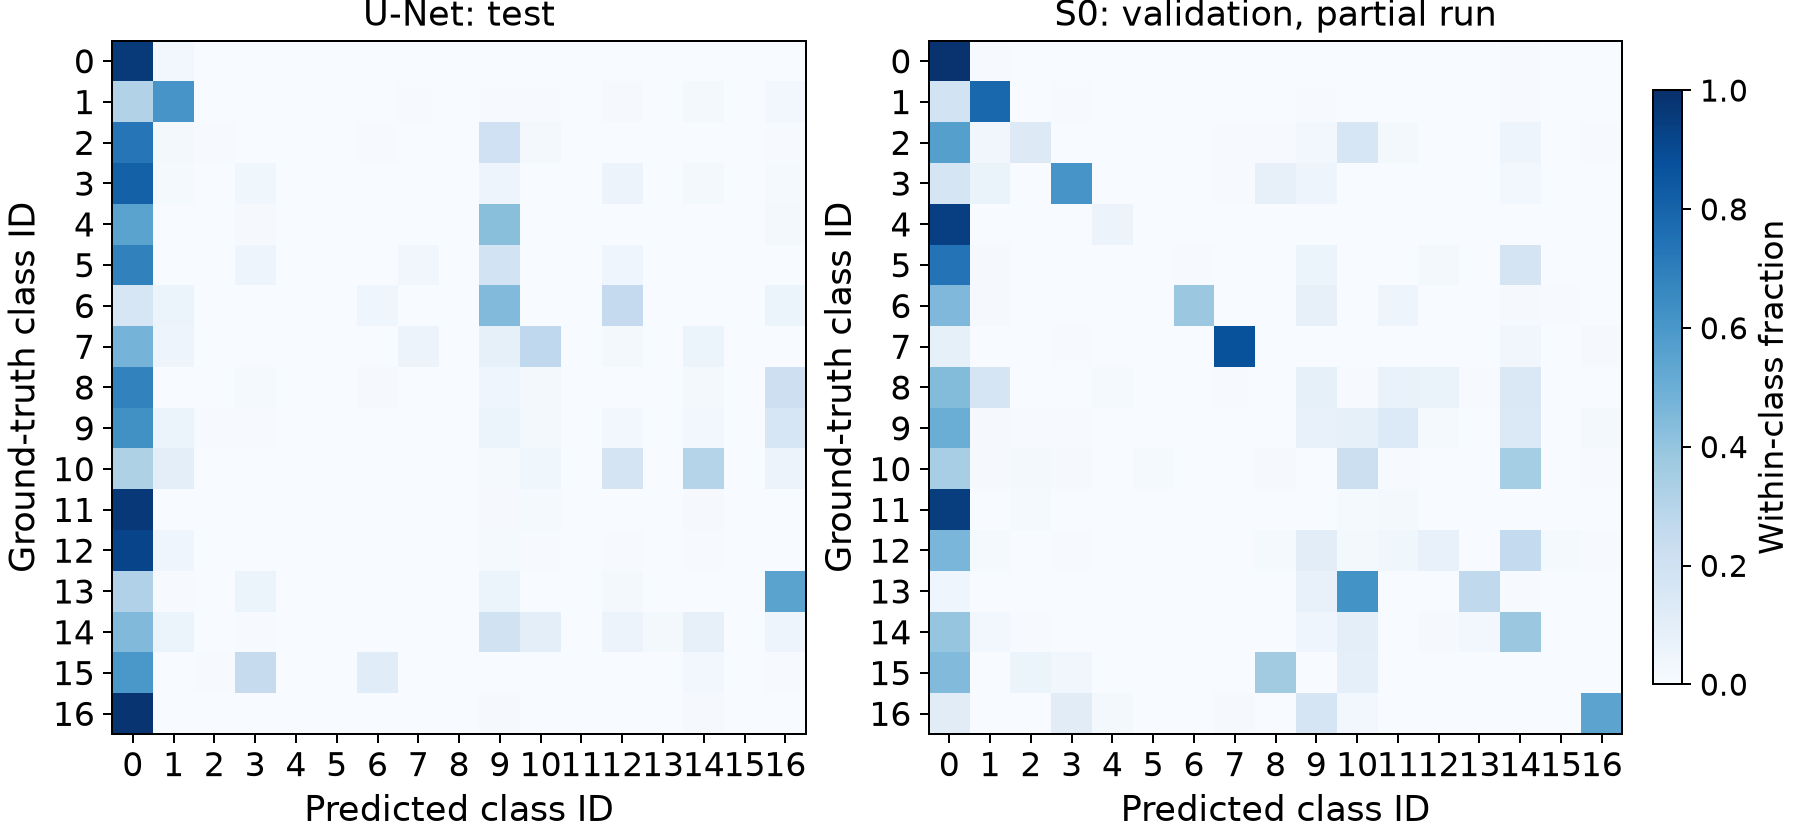
\includegraphics[width=\textwidth]{images/confusion_panels.png}
\caption{Row-normalized confusion: U-Net test (left) and partial S0 validation (right). Both color scales run 0--1; class IDs are defined in Table~\ref{tab:perclass}.}\label{fig:confusion}
\end{figure}
In the U test matrix,9,174,492 of 17,988,134 foreground pixels (51.00\%) are assigned to background. This directly measures foreground omission. It does not identify whether the missed pixels correspond to small objects, occlusion or particular visual conditions; that requires prediction-level image inspection.

\subsection{Analytical background-only reference}
A predictor that assigns every valid pixel to background provides a useful check on the interpretation of accuracy. Its confusion matrix can be constructed without inference: place each true-class support in column 0. Table~\ref{tab:background} derives this reference from the already saved held-out confusion-row totals; it is an analytical calculation on existing labels, not a newly trained model or an additional checkpoint evaluation.
\begin{table}[H]
\centering\small
\caption{Analytical constant-background reference derived from existing confusion-row supports; no model inference is required.}\label{tab:background}
\begin{tabular}{lrrrr}\toprule
Partition / predictor & Pixel acc. & FG mIoU & FG Dice & All mIoU \\ \midrule
Validation / background & 0.894015 & 0.000000 & 0.000000 & 0.052589 \\
Test / background & 0.903466 & 0.000000 & 0.000000 & 0.053145 \\
Test / U-Net & 0.894205 & 0.035627 & 0.058519 & 0.087050 \\
\bottomrule\end{tabular}
\end{table}

On test, constant background obtains pixel accuracy 0.903466, above U-Net's 0.894205, yet has foreground mIoU and Dice exactly zero. U-Net's nonzero foreground overlap and higher all-class mIoU show a different trade-off. This establishes why the study uses foreground macro metrics as primary outcomes: pixel accuracy alone can favor a predictor that never finds debris or marine-life classes.

\subsection{Compute records and qualitative evidence boundary}
S0's supplied progress log contains 15 training-phase records totaling 14,243.52 seconds (3.9565 hours) and 15 validation records totaling 838.61 seconds (13.98 minutes). These are phase durations for the 15 completed epochs, excluding setup, pilots, checkpoint writes, idle/disconnected time and final test processing. They are not complete-experiment wall time or inference latency. No inference benchmark is reported, and a completed U/S0 cost comparison is deferred until both scopes can be reconciled.

The current report includes annotation-QA overlays and aggregate confusion evidence. It does not present ground-truth overlays as model predictions. Prediction galleries, including foreground misses and inter-class confusions, will be exported from selected checkpoints after the respective run completes; no new checkpoint inference was performed during this report update.

\subsection{S1 status and the pending augmentation comparison}
S1 has a successful GPU pilot and a frozen color-on configuration, but the supplied S1 folder contains no main-run directory, epoch history or main checkpoint. Consequently there is no S1 validation/test score to compare with S0, no main-run initial-state hash pair to verify yet, and no observed augmentation effect.

The experiment remains defined as S0 versus S1 with the same architecture, initialization scheme, seed, split, optimizer, learning rate and budget. Completing this pair is the next experiment milestone; the 20-step pilot is not substituted for that comparison.
